\documentclass[a4paper,10pt]{article}

\usepackage[utf8]{inputenc}
\usepackage{t1enc}
\usepackage[spanish]{babel}
\usepackage[pdftex,usenames,dvipsnames]{color}
\usepackage[pdftex]{graphicx}
\usepackage{amsmath}
\usepackage{amsfonts}
\usepackage{amssymb}
\usepackage{listings}
\lstset{language=C}
\lstset{showstringspaces=false}
\lstset{basicstyle=\ttfamily,}

\usepackage{float}
\floatstyle{boxed} 
\restylefloat{figure}

\begin{document}


\renewcommand{\lstlistingname}{C\'odigo Fuente}
\lstloadlanguages{Octave} 
\lstdefinelanguage{MyPseudoCode}[]{Octave}{
	deletekeywords={beta,det},
	morekeywords={repmat}
} 
\lstset{
	language=MyPseudoCode,
	stringstyle=\ttfamily,
	showstringspaces = false,
	basicstyle=\footnotesize\ttfamily,
	commentstyle=\color{gray},
	keywordstyle=\bfseries,
	numbers=left,
	numberstyle=\ttfamily\footnotesize,
	stepnumber=1,                   
	framexleftmargin=0.20cm,
	numbersep=0.37cm,              
	backgroundcolor=\color{white},
	showspaces=false,
	showtabs=false,
	frame=l,
	tabsize=4,
	captionpos=b,               
	breaklines=true,             
	breakatwhitespace=false,      
	mathescape=true
}
\begin{titlepage}
        \thispagestyle{empty}
        \begin{center}
                
\includegraphics{./images/itba.jpg}
                \vfill
                \Huge{Sistemas Operativos}\\
                \vspace{1cm}
                \huge{Trabajo Práctico Especial Nº1}\\
        \end{center}
        \vspace{2cm}
        \large{
                \begin{tabular}{lcrc}
                        \textbf{Alvaro Crespo} & & 50758 & \ \ \texttt{acrespo@alu.itba.edu.ar}\\
                        \textbf{Juan Pablo Civile} & & 50453 & \ \ \texttt{jcivile@alu.itba.edu.ar}\\
                        \textbf{Darío Susnisky} & & 50592 & \ \ \texttt{dsusnisk@alu.itba.edu.ar}\\
                        \\ 
                \end{tabular}
        }
        \vfill
        \flushright{12 de Septiembre del 2011}
\end{titlepage}

\setcounter{page}{1}

\tableofcontents
\newpage
\section{Introducción}
El objetivo de este trabajo es familiarizarse con el uso de sistemas cliente-servidor concurrentes, implementando el servidor mediante la creación de procesos hijos 
utilizando \textit{fork()} y mediante la creación de \textit{threads}. Al mismo tiempo, ejercitar el uso de los distintos tipos de primitivas de sincronización y 
comunicación de procesos (IPC) y manejar con autoridad el \textit{filesystem} de Linux desde el lado usuario.

\newpage
\section{Esquema de la aplicación}

A la hora de encarar el problema en cuestión, una de las primeras cosas a plantearse era el diseño de la aplicación. Dada la naturaleza y los objetivos planteados 
para este trabajo práctico, era necesario poder identificar que partes de nuestra simulación serían modeladas como procesos y cuales tenía coherencia implementarlas 
como \textit{threads}. En este debate, también fue importante no forzar la separación de procesos cuando el problema no lo requería (por ejemplo que cada avión 
fuera un proceso independiente no agregaba nada y generaba mucha complejidad, por lo que se optó por implementarlos como \textit{threads}).\\ 

En un \textbf{primer} análisis, identificamos como potenciales procesos paralelos de nuestro programa al control del flujo principal del programa, a los parsers, 
al mapa, al \textit{output}, a las aerolíneas y a los aviones. Ya desde un comienzo nos planteamos a estos
dos últimos como threads de un mismo proceso. A continuación se puede ver un esquema de este modelo.\\

\begin{figure}[H]
\begin{center}
 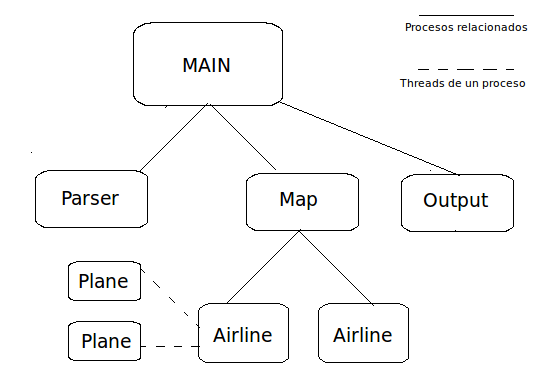
\includegraphics[scale=0.6]{./images/Diagrama_simulacion_2.png}
 % Diagrama_simulacion_2.png: 549x382 pixel, 96dpi, 14.52x10.11 cm, bb=0 0 412 286
 \caption{Esquema inicial de nuestra aplicación.}
\end{center}
\end{figure}

 Luego de cierto debate, vimos que la relación entre el flujo principal, los parsers, el \textit{output} y el mapa era demasiado fuerte, pues, 
 la combinación de estas tres cosas iban a controlar el flujo de la simulación en sí. Inclusive, estas partes tenían una secuencia bastante marcada. Así, se 
decidió que estos elementos que originalmente bien podrían haber sido planteado como procesos paralelos, era más intuitivo y coherente escribirlo como uno solo.
 Finalmente, el mapa y el \textit{output} fueron implementados como \textit{threads} del proceso principal ya que, si bien su relación es fuerte, nos resultó 
coherente que ambos puedan estar ejecutándose paralelamente.\\

Dado que las aerolíneas son independientes entre sí, ya que cada una desconoce la existencia de las demás, resulta intuitivo que cada aerolínea ejecute en un 
proceso dedicado. Como cada avión es un entidad independiente, pero a la vez es conciente de al existencia del resto de los aviones de su flota, resulta lógico 
que sean \textit{threads} dentro del proceso de su aerolínea. Esto nos permite compartir fácilmente la información entre estos y la aerolínea.

\begin{figure}[H]
\begin{center}
 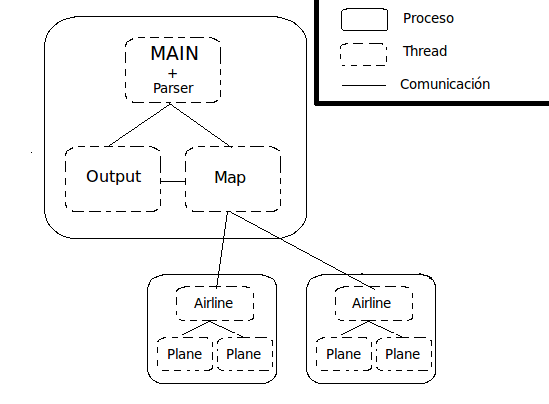
\includegraphics[scale=0.6]{./images/Diagrama_simulacion_1.png}
 % Diagrama_simulacion_1.png: 566x382 pixel, 96dpi, 14.97x10.11 cm, bb=0 0 424 286
 \caption{Esquema final de nuestra aplicación.}
\end{center}
\end{figure}

\newpage
\section{Modelo OSI}

El modelo OSI es un modelo que estandariza la forma de diseñar un programa y como comunicar diferentes programas. 
Este modelo divide una aplicación en 7 capas, donde cada capa se comunica solo con la capa "debajo".
Esto permite una clara separación de responsabilidades, llevando a un código limpio y fácilmente entedible por cualquier familiarizado con el modelo.

El sistema operativo ya provee funcionalidades compatibles con el modelo OSI, con lo cual a nuestra implementación le concierne sólo las 4 capas superiores del modelo.
Para estas 4 capas optamos por desviarnos un poco del modelo, e implementamos las capas de sesión y presentación en una sola, que llamamos capa de comunicación.

\begin{figure}[H]
\begin{center}
 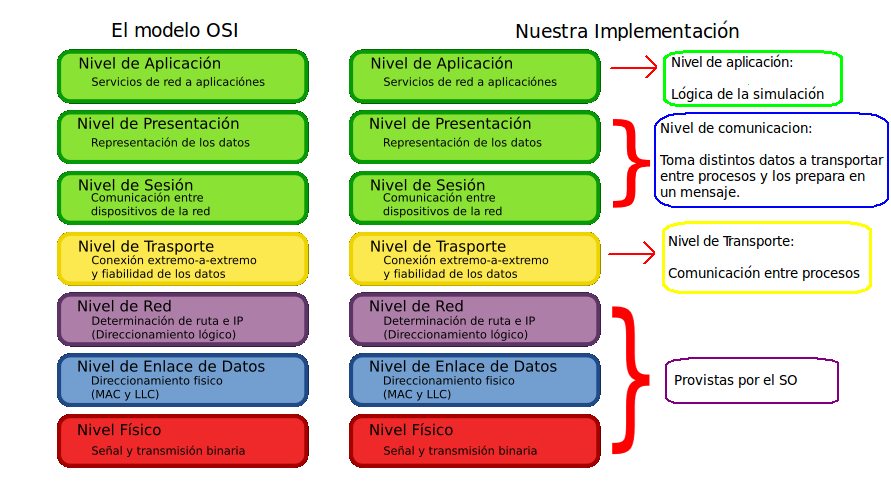
\includegraphics[scale=0.5]{./images/modelo-osi_nuestro.png}
 % modelo-osi_nuestro.png: 891x495 pixel, 96dpi, 23.57x13.10 cm, bb=0 0 668 371
 \caption{Esquema del modelo OSI y nuestra implementación del mismo.}
\end{center}
\end{figure}


\newpage
\section{Transporte}
Uno de los objetivos impuestos era utilizar diversos métodos de comunicación entre procesos, \textit{Message Queues}, \textit{Sockets}, \textit{Shared Memory} y
\textit{FIFOs}.
La consecuencia natural fue desarrollar una capa de Transporte que soportara todas estas implementaciones.
Para esto diseñamos una interfaz común a todos los métodos de \textit{IPC}.

Durante el proceso de diseño de la interfaz, pasamos por varios diseños (e implementación de los mismos) que resultaron deficientes y fueron descartados.
Nuestro primer diseño se basó fuertemente en el comportamiento de la función \textit{pipe}, ya que parecía ser la manera más simple.
O sea, el canal de comunicación entre 2 procesos se establecía antes de hacer una llamda a \textit{fork}.
Este diseño presenta varias deficiencias, entre ellas que no permite que 2 procesos que no tengan una relación padre-hijo se comuniquen.
Si bien dado el diseño de nuestra aplicación, esta restricción es aceptable, detalles de la implementación complicaban el uso de esta interfaz.
Consecuentemente, por estas complicaciones y limitaciones, optamos por descartar esta interfaz.

Antes de tomar la decisión final, evaluamos el uso de una comunicación bidireccional, donde una conexión permite la salida y entrada de mensajes, o unidireccional.
La comunicación bidireccional, presentaba la complicación de necesitar una función análoga a \textit{select}.
La implementación de esta función resultó no ser trivial para \textit{Shared Memory} y \textit{Message Queues}.
Esto llevó a que descartemos este diseño y nos llevó a nuestro diseño final, una comunicación unidireccional.

Es un diseño muy parecido al de una \textit{Message Queue}.
Cada proceso interesado en recibir mensajes, define un nombre único con el cual indentificarse a la hora de leer mensajes.
Otros procesos pueden escribir mensajes a cualquier otro proceso siempre y cuando sepan bajo que nombre escucha ese proceso.

A la hora de probar que nuestras implementaciones funcionaran correctamente, nos encontramos con que no resulta simple construir un test para esto.
La naturaleza azaroza de la ejecución de un programa multiproceso hace que un test tenga que contener muchas pruebas.
Aún más, es necesario correr este test un gran número de veces, ya que una sola ejecución no necesariamente significa que no hay errores.

Además de comunicación entre procesos, necesitabamos una manera segura de enviar mensajes entre \textit{threads}.
Para esto desarrollamos una \textit{Message Queue} utilizando herramientas de sincronización provistas por pthreads.

\newpage
\section{IPCs}
Como ya fue mencionado en la sección anterior las interfaces de los distintos tipos de IPCs eran iguales.
Sin embargo, las implementaciones fueron muy diferentes, y a la hora de escribir el código cada uno trajo
distintos tipos de problemas. El objetivo de esta sección es detallar los diferentes tipos de IPCs.
\subsection{Message Queue}

\subsection{Shared Memory}

\subsection{FIFO}
Siguiendo con la interfaz propuesta para los IPCs, el objetivo era crear un FIFO por proceso y cualquiera sea el
mensaje que se quiera transmitir, escribirlo en el FIFO del proceso receptor. Para esto, es necesario que todos los
procesos (los que esrcriben y el que lee) tengan coordinado un nombre que sera el codigo de este FIFO. Así,
al establecer una conección o al registrarse a la misma era necesario crear el FIFO tomando las precauciones necesarias
para que si el mismo ya existiese no se pise el archivo previo. Cabe destacar que los archivos FIFOS eran creado en
la carpeta \textit{temp} ya que su naturaleza es de ser archivos temporales. \\

Por otra parte, a la hora de escribir mensajes, habia que tener en cuenta que en un mismo mensaje en un FIFO, el mismo
debia contar primero con la longitud del mensaje en sí y luego con los datos que se deseaban transportar. Así, hubo
que soportar este formato generando la estructura del mensaje final para poder enviar todo en una sola escritura
asegurando así la atomicidad de la transmisión. También era necesario tener esto en cuenta en el parametro de salida 
de las funciones de lectura para poder ser consistente con los otros tipos de IPCs.
\subsection{Socket}

\newpage
\section{Comunicación}
Es importante notar que la capa de comunicación esta diseñada para abstraer lo más posible a quien la usa y que la comunicación se realiza en manera asincrónica.
Esto es, cuando se envía un mensaje que debe recibir una respuesta como consecuencia, la misma función de comunicación se encarga de enviarlo, y de esperar 
la respuesta. Lo que permite que al mirar la lógica de un avión, no sea posible darse cuenta de que es un \textit{thread} corriendo de manera independiente del mapa y
 la aerolínea. Por supuesto que esto no siempre fue posible, y en ciertos lugares de la lógica de la simulación es aparente que esta corre en diferentes procesos,
 con múltiples \textit{threads} cada uno.

\newpage
\section{Lógica de la simulación}
Para realizar la simulación en sí, comenzamos por definir como un turno de la simulación, el tiempo que tarda un avión en viajar una unidad de distancia.
Además, como se nos fue especificado, en un mismo turno un avión puede llegar a una ciudad, descargar su stock, y finalmente partir hacia otra ciudad.

Sabiendo esto, optamos por dividir el turno en 2 partes.
\begin{enumerate}
  \item los aviones que acaban de llegar a una ciudad, descargan su stock.
  \item los aviones en tránsito hacen su movimiento de una unidad de distancia.
\end{enumerate}

Y los aviones que recién descargaron, eligen su próximo destino y parten inmediatamente hacia él.

\subsection{Lógica del avión}

Una parte importante de la simulación es la lógica del avión. Esto es, como el avión ``elije'' su próximo destino. Un avión que se dirige a una ciudad en donde no 
podrá descargar nada, representa una pérdida de recursos y de tiempo de ejecución.\\

Inicialmente, nuestros aviones simplemente elegían uno de los destinos posibles que le fueran útiles, es decir a donde pudiera contribuir con algo de su stock, 
aleatoriamente. Es claro que, el avión no puede ``generar'' estos destinos posibles sino que debe recibirlos del mapa, por la restricción de que un avión no 
conoce el estado del mapa, ni el de los demás aviones.\\

Más tarde, implementamos una lógica más compleja. En ella, el avión recibía una lista de destinos en los que hubiera necesidad de las drogas que él poseía, 
ordenados por un paŕametro clave: la \textit{distancia}. De esta forma, el avión simplemente escogía siempre el primer destino, el que se encontraba más cerca, y 
se evitaban casos que reducían la perfomance. Por ejemplo, dos aviones con cargas similares, en ``puntas'' opuestas del mapa, cruzan ambos todo el mapa para ir a una 
ciudad en la otra punta, cuando podrían ir cada uno a la ciudad que se encuentra en su ``punta`` del mapa.\\

Es verdad que no hace falta que el avión reciba una lista de destinos, pudiendo recibir sólo el destino más cercano. Se decidió optar por la lista, pensando en futuras
implementaciones, con algoritmos más complejos.

\newpage
\section{Archivos de Configuración}

Los archivos de configuración, nos ayudaron a la hora de armar las estructuras de datos en las que almacenaríamos posteriormente toda la información que la 
aplicación requería. Una de las cosas que nos hizo ver anticipadamente, fue el hecho de que, para evitar \textit{redundancia de información}, podíamos tener 
una colección de las drogas, y que las estructuras almacenen solamente \textit{referencias} a ellas. 

Uno de los primeros problemas con los que nos topamos, fue el hecho de que los archivos de configuración de los cuales la aplicación debía levantar la información,
 tenían un formato bastante díficil para trabajar con el lenguaje C. Al no contar con una estructura que pueda ir agregando elementos a una colección y cambiando 
de tamaño dinámicamente, debimos implementar nuestra propia estructura, \textit{Vector}. Esto probó ser muy útil más adelante, ya que la utilizamos en otros sectores 
del programa.\\

Otro problema con el formato de los archivos de configuración, fue que los límites de las ``iteraciones'' se marcaban con líneas en blanco, y al parecer hay 
problemas al querer leer el $\backslash n$ con $fscanf$. Para lidiar con esta situación, recurrimos a la única solución que encontramos, aunque en términos de 
código no es muy elegante.\\

\newpage
\section{Output}

Como ya se bien se dijo, le asignamos la responsabilidad de imprimir a pantalla a un \textit{thread} del proceso principal, el \textit{Output}. \\

Al pensar en esta sección nos dimos cuenta que se podría utilizar tranquilamente la función \textit{printf}, por más que no fuera \textit{thread-safe},
 ya que después de todo solo un \textit{thread} iba a ejecutarla. Pronto, desechamos esa opción por la simple razón de que no queríamos tener que obligar al usuario 
de la aplicación a scrollear la pantalla. Por esta razón pensamos en tener un \\textit{layout} estático e ir actualizando la pantalla.\\
Para lograr este objetivo, decicidimos utilizar librería \textit{ncurses}, la cual nos facilitó el trabajo a la hora de imprimir la información en un sector específico
de la pantalla y de actualizarla.\\

Para comunicar a este \textit{thread} con el mapa, utilizamos la estructura \textit{Message Queue} que implementamos, de forma similar al uso que le dimos 
para comunicar a los \textit{avión} con la aerolínea.\\

De nuevo, se presentó el problema de la sincronización, en este caso con el mapa, ya que es claro que las operaciones relacionadas con la pantalla consumen más 
tiempo. No nos pareció correcto que haya un desfasaje entre el \textit{Output} y el mapa. Es decir, que en pantalla se muestre la información del turno 12, 
cuando el mapa en realidad va por el turno 23. Por esta razón, utilizamos un semáforo para resolver este problema y lograr una correcta sincronización.

\newpage
\section{Conclusiones}

Queda claro que este trabajo podría haberse realizado sin necesidad de recurrir al procesamiento paralelo y a la comunicación entre procesos. Pero al haberlo 
hecho de de esta forma, la experiencia adquirida y el aprendizaje resulta mucho más significativo. Por varias razones:

\begin{itemize}
\item la experiencia adquirida al trabajar con varios procesos corriendo al mismo tiempo, al igual que varios \textit{threads}.
\item la comunicación entre estos procesos.
\item la separación en capas, consecuencia necesaria, que agrega mucha claridad al código y conceptualmente, al diferenciar claramente las responsabilidades.
\item la familiarización con los estándares \textit{POSIX} y \textit{System V}, o el simple de hecho de trabajar contra interfaces predefinidas y respetando
      un estándar predefinido.
\end{itemize}

Con respecto al uso de \textit{threads}  y procesos, nos topamos con una fuerte diferencia entre utilizar unos y otros. Por ejemplo, el uso de variables globales 
en un \textit{thread} debe ser llevado a cabo con mucho cuidado, ya que el estado global, o \textit{Data Segment}, es compartido por los demás \textit{threads} 
del mismo proceso. Esto no es así con los procesos, cuyo estado global es propio y solo visible a ellos mismos. Por suerte, el \textit{stack} no es compartido 
por distintos \textit{threads} los que les da un cierto grado de independencia, para que realicen distinas tareas. Otra diferencia que notamos, tiene que ver 
con la sincronizacíon. Mientras que un simple \textit{lock} de un \textit{mutex} en la mayoría de los casos era lo único que se debía hacer para sincronizar 
\textit{threads}, para procesos se requirió el uso de técnicas más avanzadas como semáforos.

Por otra parte, fue muy interesante durante el desarrollo de la aplicación los conocimientos adquiridos sobre \textit{deadlocks}.
Si bien al comenzar, estos eran un problema que nos costaba mucho identificar. Con el tiempo y la experiencia nos vimos mas cómodos
a la hora de prevenir \textit{deadlocks} e inclusive a la hora de darnos cuenta que estábamos cayendo en uno. Por la naturaleza de este
problema es imposible salir de un \textit{deadlock} y por eso es que es necesario ser cuidadoso a la hora de escribir el
código y prevenirlos lo más posible.

Una vez terminado el trabajo, surgió la pregunta de cual era la implementación de IPC más rápida. Como nos dimos cuenta más tarde, esto no es tan fácil de determinar. 
Esto se debe a que el rendimiento de cada implementación varía dependiendo de la ejecución debido al procesamiento paralelo, el cual no es determínistico. 
Es decir, no siempre se reproduce exactamente la misma ejecución dadas las mismas condiciones iniciales. \\

Para observar la perfomance de la aplicación, utilizamos 4 simulaciones distintas:

\begin{table}[H]
\begin{center}
\begin{tabular}{l|l|l|l}
Nº & Ciudades & Aerolíneas & Aviones \\
\hline
1 & 5 & 2 & 8 \\
2 & 5 & 1 & 3 \\
3 & 10 & 10 & 40 \\
4 & 50 & 10 & 50 \\
\end{tabular}
\caption{Características de las simulaciones}
\end{center}
\end{table}

Usando estas 4 simulaciones, procedimos a tomar el tiempo promedio de una ejecución al realizar 100 iteraciones consecutivas de cada simulación.
Cabe aclarar que estas simulaciones fueron ejecutadas con un \textit{output} minimo, minimizando así sus tiempos.

\begin{figure}[H]
\begin{center}
 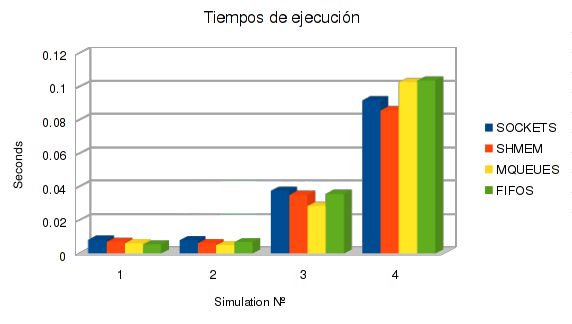
\includegraphics[scale=0.75]{./images/runningTimesChart.png}
 % runningTimesChart.png: 572x324 pixel, 96dpi, 15.13x8.57 cm, bb=0 0 429 243
  \caption{Comparación de los tiempos de ejecución de cada implementación.}
\end{center}
\end{figure}

En base a estos datos, pudimos concluir que en general la de \textit{shared memory} es la implementación con mejores tiempos, seguido de la de \textit{socket}. 
Aunque, como puede observarse, para las primeras simulaciones, las menos intensivas, las implementaciones de \textit{message queues} y \textit{FIFOs} parecen 
tener mejores tiempos. Después de analizar los datos, nuestra explicación es que, en esos casos el mayor \textit{overhead} que tienen las implementaciones como 
\textit{socket} y \textit{shared memory}, hacen que sus tiempos de ejecución sean levemente mayores. 
Pero, para simulaciones más intensivas, como por ejemplo la número 4, ese \textit{overhead} se torna despreciable, revelando los resultados que se observan en 
el gráfico: esas implementaciones terminan siendo más rápidas para problemas más complejos.\\

\newpage     
\section{Referencias}

\begin{itemize}
  \item Material provisto por la cátedra.
  \item UNIX system programming. Second Edition. Keith Havilland, Dina Gray, Ben Salama.
  \item http://cplusplus.com/cir
  \item http://beej.us/guide/bgipc/output/html/multipage/unixsock.html
  \item https://computing.llnl.gov/tutorials/pthreads/
  \item https://computing.llnl.gov/tutorials/parallel\_comp/
  \item http://www.csc.villanova.edu/~mdamian/threads/posixsem.html
  \item http://www.cs.cf.ac.uk/Dave/C/node25.html
  \item http://www.users.pjwstk.edu.pl/~jms/qnx/help/watcom/clibref/mq\_overview.html
  \item http://linux.die.net/man/7/mq\_overview
\end{itemize}
   
\end{document}
